\documentclass[10pt]{article}

\usepackage{adjustbox}
\usepackage{amsmath}
\usepackage[french, onelanguage]{algorithm2e}
\usepackage[utf8]{inputenc}
\usepackage[french]{babel}
\usepackage{csquotes}
\usepackage[T1]{fontenc}
\usepackage{geometry}
\usepackage{glossaries}
\usepackage{graphicx}
\usepackage[hidelinks]{hyperref}
\usepackage[utf8]{inputenc}
\usepackage{listings}
\usepackage{lstautogobble}
\usepackage{tabularx}
\usepackage{textcase}
\usepackage{tikz}
\usepackage{tocloft}
\usepackage{verbatim}
\usepackage{xcolor}
\usepackage{fancyhdr}
%\usepackage[pdf]{pstricks}
%\usepackage{auto-pst-pdf}
%\usepackage{uml}

\makeglossaries


\usetikzlibrary{calc, shapes.multipart, chains, arrows}

\definecolor{RoyalBlue}{cmyk}{1, 0.50, 0, 0}

\lstset{language=C++,
  keywordstyle=\color{RoyalBlue},
  basicstyle=\scriptsize\ttfamily,
  commentstyle=\ttfamily\itshape\color{darkgray},
  stringstyle=\ttfamily,
  breaklines=true,
  keepspaces=true,
  numbers=left,
  numbersep=5pt,
  showspaces=false,
  showstringspaces=false,
  showtabs=false,
  tabsize=4,
  autogobble=true
}

\geometry{
  a4paper,
  total={170mm,237mm},
  left=20mm,
  top=30mm,
}

\pagestyle{fancy}
\setlength{\headheight}{55.6pt}
\addtolength{\topmargin}{-43.6pt}
\setlength{\footskip}{60pt}
\fancyhf{}
\rhead{
\includegraphics[width=4cm]{pictures/header.jpg}}
\rfoot{
\includegraphics[width=4cm]{pictures/footer.jpg}}

\begin{document}

\begin{titlepage}
	\centering
	\vspace*{\fill}
	\begin{center}
		\Huge 
		\textbf{Sokoban}\\
		\vspace*{0.5cm}
		\large
		\textit{Giorgio Caculli LA196672, Guillaume Lambert LA198116, Tanguy Taminiau LA199566, Nathan Thaon LA188132 \\ Groupe B01}
		\vspace*{0.5cm}
		\\ \today
	\end{center}
	\vspace*{\fill}
	\thispagestyle{fancy}
\end{titlepage}	

\newpage
\tableofcontents

\newpage
\section{Introduction}
Dans le cadre du cours de développement de jeux vidéo de l'UE 308, nous avons dû créer un jeu de manière autonome.
L'objectif pédagogique de ce projet est de pousser l'élève à mieux appréhender la programmation en C++ vue au cours ainsi que d'apprendre à utiliser une librairie graphique en C++.
De plus, la grande liberté accordée à ce projet oblige l'élève à apprendre à se documenter, savoir faire des recherches.
L'objectif du projet est simple, créer un jeu selon notre propre envie.
\section{Présentation du sujet}
Notre jeu sera un jeu de type puzzle. Il sera en vue 2D, vue du haut. Le but du jeu sera d’atteindre un objectif, en se frayant un chemin via la résolution d’un puzzle. 
La mécanique principale de ce jeu sera de pouvoir pousser une caisse pour nous permettre d’atteindre notre objectif qui sera de pousser ces caisses sur certains points pour terminer le niveau. 
Les mouvements du personnage et des caisses se feront en case par case et les caisses ne pourront pas être poussées deux par deux. Il y aura aussi la présence d’un compteur de mouvements et  un 
un compteur de reset.

\subsection{Spécification technique}
\subsubsection{GUI : SFML}
\begin{figure}[h]
	\centering
	
\includegraphics{pictures/SFML_logo.png}
	\caption{Logo SFML}
	\label{fig:logo_sfml}
\end{figure}
SFML est une librairie qui donne accès à une vaste variété de fonctionnalités purement écrites en C++. Les cinq fonctionnalités dont nous disposons sont les gestions suivantes:
\begin{itemize}
	\item Toute interaction avec le système d'exploitation
	\item Fenêtrage
	\item Graphismes
	\item Son
	\item Réseau
\end{itemize}

SFML permet le cross-platforming : un logiciel codé avec SFML aura le même visuel indépendamment du système d'exploitation sur lequel le jeu tourne.

\subsubsection{Librairie Boost}
\begin{figure}[h]
	\centering
	
\includegraphics[width=0.5\textwidth]{pictures/Boost_logo.png}
	\caption{Logo Boost}
	\label{fig:logo_boost}
\end{figure}
La librairie de logging que nous utiliserons se nomme Boost. En quelques mots, la librairie Boost est elle-même un ensemble de librairies permettant d'étendre les fonctionnalités de C++. Dans notre cas, nous utiliserons les fonctionnalités prédéfinies de Boost. Notamment Log, qui nous donne accès à la possibilité d'enregistrer les différentes interactions qui ont eu lieu lors de l'exécution du jeu.

\subsubsection{Fichiers}
Les niveaux et les sauvegardes seront stockés dans des fichiers purement textuels. Ces fichiers ne stockeront que le design des niveaux ou de la partie en cours.
Comme déclaré précédemment, Boost est un ensemble de librairies, dans cet ensemble il existe la librairie Boost.JSON. Grâce à cette librairie, nous serons capable de stocker des informations en format JSON, comme par exemple, une liste des scores.

\subsubsection{OS}
Les systèmes d'exploitation sur lesquels nous testerons notre jeu sont les suivants:
\begin{itemize}
	\item Linux
	\item MS Windows 10
	\end{itemize}
%Étant donné que toutes les librairies citées précédemment sont cross-platform, nous pouvons assurer que notre jeu sera entièrement cross-platform.

\section{Analyse}
\subsection{Product Backlog}

\noindent\adjustbox{max width=\textwidth}{
\begin{tabular}{| p{1cm} | p{16cm} |}
	\hline
	US-01 & En tant qu'utilisateur je voudrais reset une partie.\\
	\hline
	US-02 & En tant qu'utilisateur je voudrais mettre en pause la partie.\\
	\hline
	US-03 & En tant qu'utilisateur je voudrais sauvegarder une partie.\\
	\hline
	US-04 & En tant qu'utilisateur je voudrais charger des niveaux personnalisé.\\
	\hline
	US-05 & En tant qu'utilisateur je voudrais arrêter mon jeu à tout môment.\\
	\hline
	US-06 & En tant qu'utilisateur je voudrais une musique de fond.\\
	\hline
	US-07 & En tant qu'utilisateur je voudrais gérer le volume de la musique et des effets.\\
	\hline
	US-08 & En tant qu'utilisateur je voudrais créer des niveaux personnaliser.\\
	\hline
\end{tabular}
}

\newpage
\section{diagramme}
\subsection{Diagramme UML}
\begin{figure}[h]
	\centering
	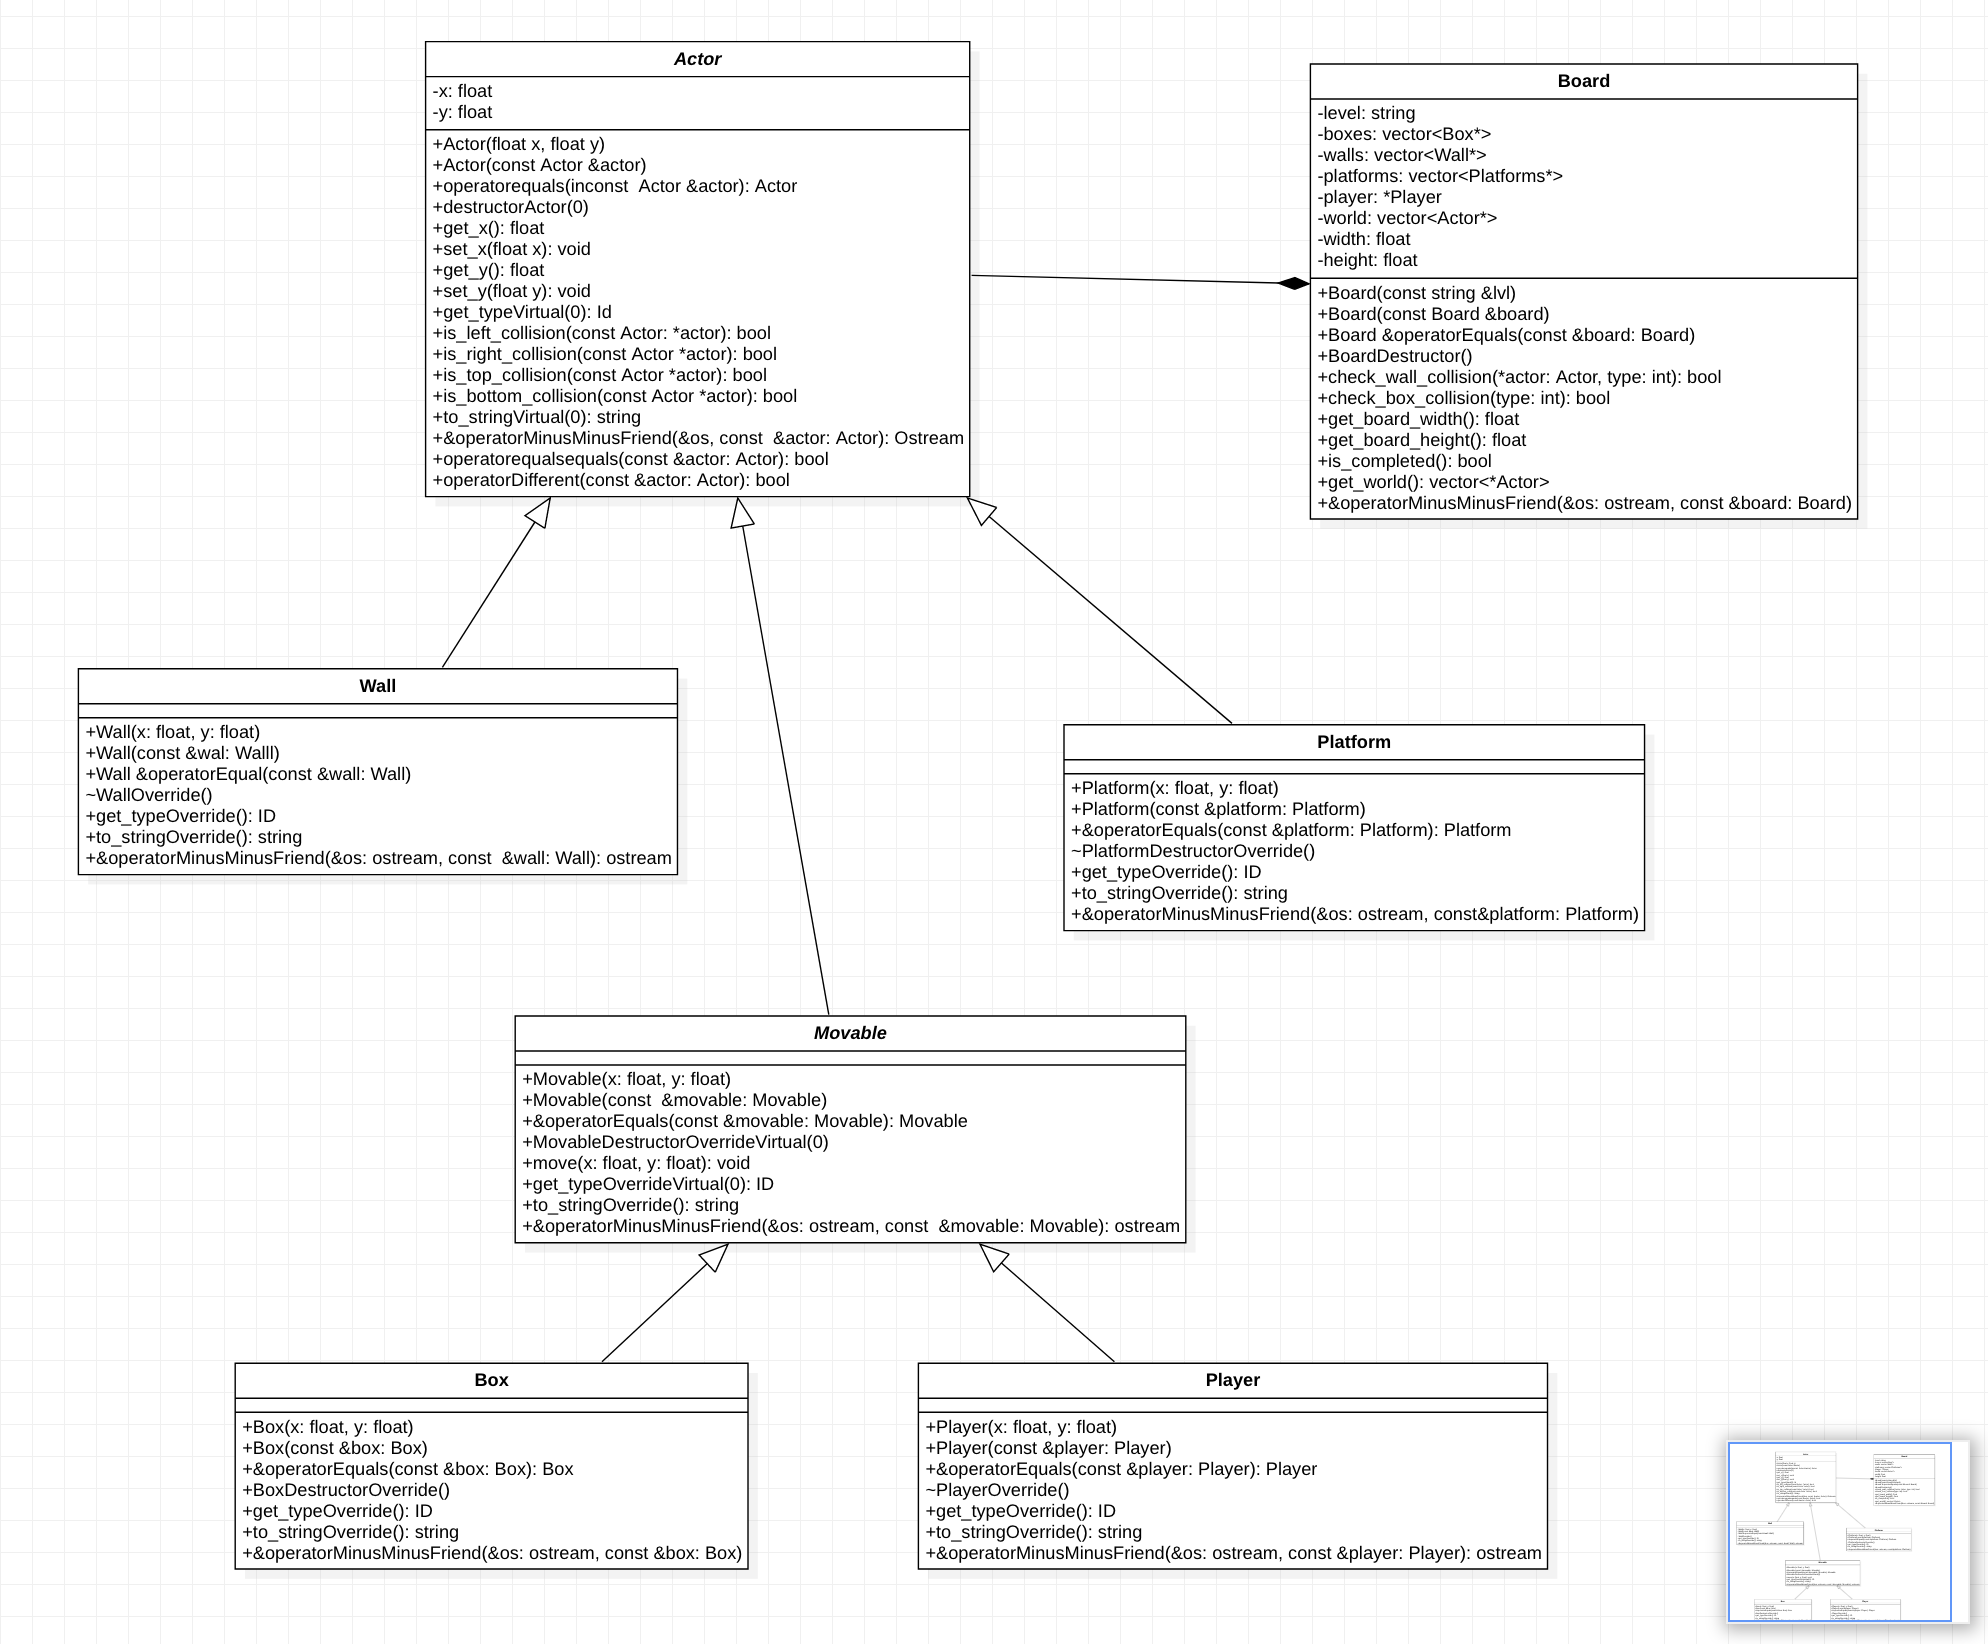
\includegraphics[width=\textwidth] {pictures/uml.png}
	\caption{diagramme de classe}
	\label{fig:UML}
\end{figure}
La Board est composé d'Actor ou de ses spécialisations. Plus précisement, une board est composé d'objet immobile tels que des Walls et des Platforms mais aussi d'objet mobile tels que des Box et un personnage.

\newpage
\subsection{Diagramme d'activité}
\begin{figure}[h]
	\centering
	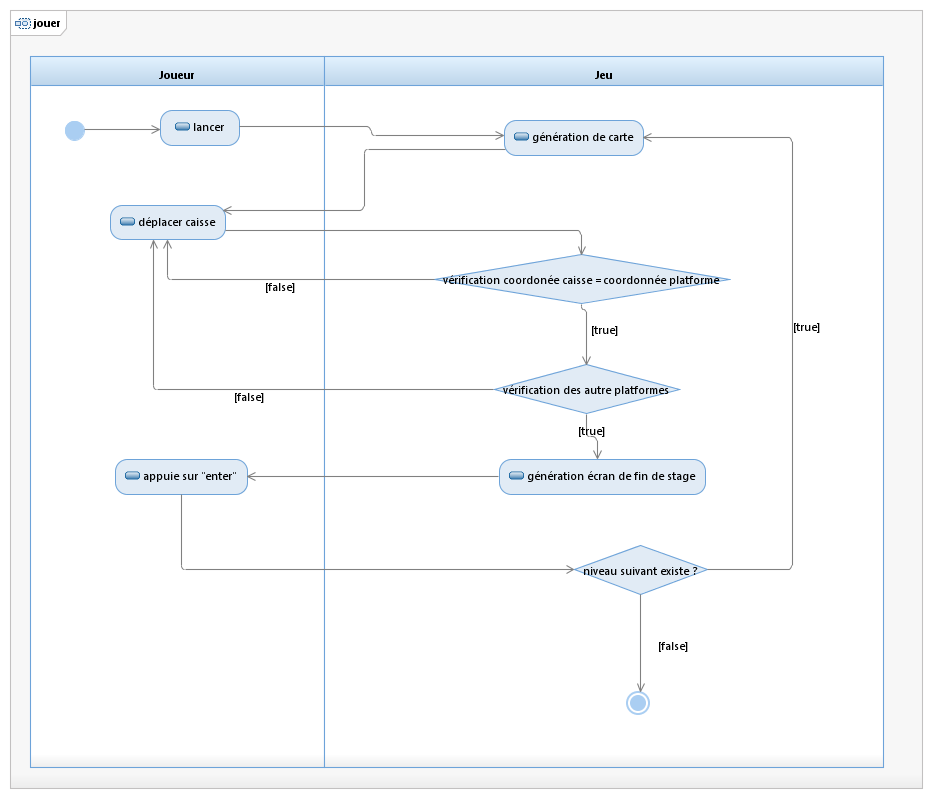
\includegraphics[width=\textwidth] {pictures/dia_activite_jouer.png}
	\caption{diagramme d'activité}
	\label{fig:diagramme_activite}
\end{figure}

\newpage
\subsection{Diagramme Design Pattern State}
\begin{figure}[h]
	\centering
	\includegraphics[width=\textwidth] {pictures/state.png}
	\caption{diagramme du design pattern state}
	\label{fig:diagramme_design_pattern_state}
\end{figure}
\newpage
\section{Code source}

\subsection{Aspect Intéressant}
Un aspect intéressant qui a demandé beaucoup de recherché était de réussir à mettre en place la randomisation des différents aspects graphiques présents sur la carte.
Afin de rendre le jeu plus varié, différentes algorithmes propres à C++ ont été exploité.
Pour créer un niveau de randomisation, C++ demande à mettre en place un générateur de \enquote{seed} qui permettra par la suite de choisir de manière aléatoire entre les différentes choix proposés dans les énumérations des couleurs.
Pour ce faire, on a exploité le \enquote{mersenne twister engine}, aussi connu en C++ sous le nom de \enquote{mt19937}.
Ce mécanisme permet de retourner un entier de la taille maximale de 32 bit, en partant d'un seed randomiquement généré.
C'est grâce à toutes ses engine qu'on a su avoir une complète randomisation des assets lors de l'affichage de la carte.

\subsection{Main}
\subsubsection{main.hpp}
\lstinputlisting{../../src/main.hpp}
\subsubsection{main.cpp}
\lstinputlisting{../../src/main.cpp}

\subsection{Model}
\subsubsection{Actor.hpp}
\lstinputlisting{../../src/model/Actor.hpp}
\subsubsection{Actor.cpp}
\lstinputlisting{../../src/model/Actor.cpp}
\subsubsection{Movable.hpp}
\lstinputlisting{../../src/model/Movable.hpp}
\subsubsection{Movable.cpp}
\lstinputlisting{../../src/model/Movable.cpp}
\subsubsection{Box.hpp}
\lstinputlisting{../../src/model/Box.hpp}
\subsubsection{Box.cpp}
\lstinputlisting{../../src/model/Box.cpp}
\subsubsection{Platform.hpp}
\lstinputlisting{../../src/model/Platform.hpp}
\subsubsection{Platform.cpp}
\lstinputlisting{../../src/model/Platform.cpp}
\subsubsection{Player.hpp}
\lstinputlisting{../../src/model/Player.hpp}
\subsubsection{Player.cpp}
\lstinputlisting{../../src/model/Player.cpp}
\subsubsection{Wall.hpp}
\lstinputlisting{../../src/model/Wall.hpp}
\subsubsection{Wall.cpp}
\lstinputlisting{../../src/model/Wall.cpp}
\subsubsection{Board.hpp}
\lstinputlisting{../../src/model/Board.hpp}
\subsubsection{Board.cpp}
\lstinputlisting{../../src/model/Board.cpp}

\subsection{Util}
\subsubsection{Logger.hpp}
\lstinputlisting{../../src/util/Logger.hpp}
\subsubsection{Logger.hpp}
\lstinputlisting{../../src/util/Logger.cpp}

\subsection{UI}
\subsubsection{Category.hpp}
\lstinputlisting{../../src/ui/Category.hpp}
\subsubsection{Menu.hpp}
\lstinputlisting{../../src/ui/Menu.hpp}
\subsubsection{Menu.cpp}
\lstinputlisting{../../src/ui/Menu.cpp}
\subsubsection{Resource\_Holder.hpp}
\lstinputlisting{../../src/ui/Resource_Holder.hpp}
\subsubsection{Resource\_Holder.inl}
\lstinputlisting{../../src/ui/Resource_Holder.inl}
\subsubsection{Utility.inl}
\lstinputlisting{../../src/ui/Utility.inl}

\subsection{GUI}
\subsubsection{Resource\_Identifiers.hpp}
\lstinputlisting{../../src/ui/gui/Resource_Identifiers.hpp}
\subsubsection{Animation.hpp}
\lstinputlisting{../../src/ui/gui/Animation.hpp}
\subsubsection{Animation.cpp}
\lstinputlisting{../../src/ui/gui/Animation.cpp}
\subsubsection{Application.hpp}
\lstinputlisting{../../src/ui/gui/Application.hpp}
\subsubsection{Application.cpp}
\lstinputlisting{../../src/ui/gui/Application.cpp}
\subsubsection{Music\_Player.hpp}
\lstinputlisting{../../src/ui/gui/Music_Player.hpp}
\subsubsection{Music\_Player.cpp}
\lstinputlisting{../../src/ui/gui/Music_Player.cpp}
\subsubsection{Scene\_Node.hpp}
\lstinputlisting{../../src/ui/gui/Scene_Node.hpp}
\subsubsection{Scene\_Node.cpp}
\lstinputlisting{../../src/ui/gui/Scene_Node.cpp}
\subsubsection{Sound\_Node.hpp}
\lstinputlisting{../../src/ui/gui/Sound_Node.hpp}
\subsubsection{Sound\_Node.cpp}
\lstinputlisting{../../src/ui/gui/Sound_Node.cpp}
\subsubsection{Sound\_Player.hpp}
\lstinputlisting{../../src/ui/gui/Sound_Player.hpp}
\subsubsection{Sound\_Player.cpp}
\lstinputlisting{../../src/ui/gui/Sound_Player.cpp}
\subsubsection{Sprite\_Node.hpp}
\lstinputlisting{../../src/ui/gui/Sprite_Node.hpp}
\subsubsection{Sprite\_Node.cpp}
\lstinputlisting{../../src/ui/gui/Sprite_Node.cpp}
\subsubsection{Utility.hpp}
\lstinputlisting{../../src/ui/gui/Utility.hpp}
\subsubsection{Utility.cpp}
\lstinputlisting{../../src/ui/gui/Utility.cpp}
\subsubsection{World.hpp}
\lstinputlisting{../../src/ui/gui/World.hpp}
\subsubsection{World.cpp}
\lstinputlisting{../../src/ui/gui/World.cpp}

\subsection{Components}
\subsubsection{Component.hpp}
\lstinputlisting{../../src/ui/gui/components/Component.hpp}
\subsubsection{Component.cpp}
\lstinputlisting{../../src/ui/gui/components/Component.cpp}
\subsubsection{Container.hpp}
\lstinputlisting{../../src/ui/gui/components/Container.hpp}
\subsubsection{Container.cpp}
\lstinputlisting{../../src/ui/gui/components/Container.cpp}
\subsubsection{Button.hpp}
\lstinputlisting{../../src/ui/gui/components/Button.hpp}
\subsubsection{Button.cpp}
\lstinputlisting{../../src/ui/gui/components/Button.cpp}
\subsubsection{Label.hpp}
\lstinputlisting{../../src/ui/gui/components/Label.hpp}
\subsubsection{Label.cpp}
\lstinputlisting{../../src/ui/gui/components/Label.cpp}

\subsection{Entities}
\subsubsection{Entity.hpp}
\lstinputlisting{../../src/ui/gui/entities/Entity.hpp}
\subsubsection{Entity.cpp}
\lstinputlisting{../../src/ui/gui/entities/Entity.cpp}
\subsubsection{Entity\_Box.hpp}
\lstinputlisting{../../src/ui/gui/entities/Entity_Box.hpp}
\subsubsection{Entity\_Box.cpp}
\lstinputlisting{../../src/ui/gui/entities/Entity_Box.cpp}
\subsubsection{Entity\_Movable.hpp}
\lstinputlisting{../../src/ui/gui/entities/Entity_Movable.hpp}
\subsubsection{Entity\_Movable.cpp}
\lstinputlisting{../../src/ui/gui/entities/Entity_Movable.cpp}
\subsubsection{Entity\_Platform.hpp}
\lstinputlisting{../../src/ui/gui/entities/Entity_Platform.hpp}
\subsubsection{Entity\_Platform.cpp}
\lstinputlisting{../../src/ui/gui/entities/Entity_Platform.cpp}
\subsubsection{Entity\_Player.hpp}
\lstinputlisting{../../src/ui/gui/entities/Entity_Player.hpp}
\subsubsection{Entity\_Player.cpp}
\lstinputlisting{../../src/ui/gui/entities/Entity_Player.cpp}
\subsubsection{Entity\_Wall.hpp}
\lstinputlisting{../../src/ui/gui/entities/Entity_Wall.hpp}
\subsubsection{Entity\_Wall.cpp}
\lstinputlisting{../../src/ui/gui/entities/Entity_Wall.cpp}

\subsection{States}
\subsubsection{State\_Identifiers.hpp}
\lstinputlisting{../../src/ui/gui/states/State_Identifiers.hpp}
\subsubsection{State.hpp}
\lstinputlisting{../../src/ui/gui/states/State.hpp}
\subsubsection{State.cpp}
\lstinputlisting{../../src/ui/gui/states/State.cpp}
\subsubsection{State\_Game.hpp}
\lstinputlisting{../../src/ui/gui/states/State_Game.hpp}
\subsubsection{State\_Game.cpp}
\lstinputlisting{../../src/ui/gui/states/State_Game.cpp}
\subsubsection{State\_Menu.hpp}
\lstinputlisting{../../src/ui/gui/states/State_Menu.hpp}
\subsubsection{State\_Menu.cpp}
\lstinputlisting{../../src/ui/gui/states/State_Menu.cpp}
\subsubsection{State\_Pause.hpp}
\lstinputlisting{../../src/ui/gui/states/State_Pause.hpp}
\subsubsection{State\_Pause.cpp}
\lstinputlisting{../../src/ui/gui/states/State_Pause.cpp}
\subsubsection{State\_Settings.hpp}
\lstinputlisting{../../src/ui/gui/states/State_Settings.hpp}
\subsubsection{State\_Settings.cpp}
\lstinputlisting{../../src/ui/gui/states/State_Settings.cpp}
\subsubsection{State\_Stack.hpp}
\lstinputlisting{../../src/ui/gui/states/State_Stack.hpp}
\subsubsection{State\_Stack.cpp}
\lstinputlisting{../../src/ui/gui/states/State_Stack.cpp}
\subsubsection{State\_Title.hpp}
\lstinputlisting{../../src/ui/gui/states/State_Title.hpp}
\subsubsection{State\_Title.cpp}
\lstinputlisting{../../src/ui/gui/states/State_Title.cpp}

\section{Implémentation}
Présentation du programme et capture d'écran

\newpage
\section{Contribution}
Partie de la doc sur la contribution de chaque personne sur le projet

Giorgio a réalisé l'interface graphique. Etant plus en avance que les autres sur le language C++, il s'est directement attaqué à l'interface graphique donc de la matière qui n'a pas été vue, étant donné que Giorgio avait déjà vu une partie de la matière de C++. états du jeu
\\

Tanguy a réalisé  l'UML de base pour mettre en place le début du projet, celui-ci a été appelé à évoluer avec le developpement du projet. Tanguy suite au développement de l'UML a commencé l'écriture des différentes classes du modèle.\\

Guillaume a réalisé une partie de l'algorithmique du modèle, notamment la gestion des collisions. Guillaume a aussi aidé en naviguant entre les différents participants du projet en fonction de là où il serait le plus utile.\\

Nathan : ...

\section{Conclusion}
Ce projet nous permit de nous rendre compte de ce qu'est un projet de création de jeu vidéo.
Cela nous a aussi permit de nous familiariser avec le language de programmation C++ mais aussi le logiciel de version git.
De plus, nous avons appris à bien communiquer et s'organiser entre collègues/coéquipiers.
Ce projet nous a permis aussi d'apprendre à combiner ce que nous apprenons en cours avec de la recherche de documentation sur internet.
En finalité, nous sommes contents du résultat obtenu actuellement, cependant, nous pensons arrivez plus loin et avons légèrement sous estimé le temps nécessaire pour le jeu initialement prévu.
Nous tenons à remercier ceux qui nous donné leurs avis par rapport au design du jeu.
Et nous tenons à remercier particulièrement Mr. Altares pour ses bons conseils.

\section{Bibliographie}
Partie abritant la bibliographie


%\newpage
%\printglossary

\end{document}
